\section{Experiment 1: Single Linear Node on a 2D Gaussian}
\label{sec:experiment1}

In this experiment, we investigate whether single linear-node neural networks with either absolute value (Abs) or rectified linear unit (ReLU) activation functions can learn to approximate the Mahalanobis distance in a 2D Gaussian distribution. Specifically, we aim to determine if these simple models capture the principal components of the Gaussian distribution, as predicted by our theoretical framework.

\subsection{Methodology}

We generated a synthetic dataset from a bivariate Gaussian distribution. The dataset $X$ was used to compute the true Mahalanobis distance for each point Equation~\eqref{eq:mahalanobis_distance}. These distances served as the target outputs $y$ for training the models.

Each model consisted of a single linear unit followed by either a ReLU or Abs activation function. Weights were initialized using Xavier initialization. To ensure diverse initial conditions, we selected a random point $\mathbf{z} \in \mathbb{R}^2$ uniformly from $[-8, 8]^2$ and set the bias as:

\begin{equation} b = -\mathbf{W} \mathbf{z}, \end{equation}

so that the decision boundary (defined by $\mathbf{W} \mathbf{x} + b = 0$) passes through the point $\mathbf{z}$. This strategy ensures that the initial decision boundaries are distributed throughout the input space.

To prevent dead ReLU nodes (nodes that output zero for all inputs), we checked the initial activations and reinitialized any models where this occurred.

Setup and training parameters are summarized in Table~\ref{tab:config_params}.

\begin{table}[h]
\centering
\caption{Configuration Parameters}
\label{tab:config_params}
\begin{tabular}{ll}
\hline
Parameter & Value \\
\hline
Activation Functions & ReLU, Abs \\
Loss Function & Mean Squared Error (MSELoss) \\
Optimizer & SGD \\
Learning Rate & 0.001 \\
Epochs & 200 \\
Momentum & 0.9 \\
Weight Initialization & Xavier Initialization \\
Bias Initialization & $b = -\mathbf{W} \mathbf{z}$, $\mathbf{z} \sim \mathcal{U}([-8,8]^2)$ \\
Number of Models & 300 per activation function \\
Number of Data Points & 1024 \\
Mean Vector $\boldsymbol{\mu}$ & $[3.0, 2.0]^\top$ \\
Covariance Matrix $\boldsymbol{\Sigma}$ & $\begin{bmatrix} 2.0 & -1.0 \\ -1.0 & 1.0 \end{bmatrix}$ \\
\hline
\end{tabular}
\end{table}

\subsection{Objectives and Hypotheses}

Based on our theoretical framework, we hypothesize the following:

\begin{enumerate} 
    \item \textbf{Abs Activation Hypothesis}: Models using the Abs activation function will learn to approximate the Mahalanobis distance by aligning their weights the largest principal component of the Gaussian distribution. This alignment should result in lower error compared to models using ReLU activations.
    \item 
    \item \textbf{ReLU Activation Hypothesis}: Models using the ReLU activation function are less likely to align with the principal components due to the asymmetry of the ReLU function, potentially resulting in higher error. However, studying their solution space may provide insights into how ReLU models approximate the distance function.
\end{enumerate}

\subsection{Results and Discussion}

\subsubsection{Visualization of Learned Weights}

To analyze the learned models, we visualized the weights $\mathbf{W}$ by representing them as vectors originating from the projection of the mean vector $\boldsymbol{\mu}$ onto the model's decision boundary. Specifically, for each model, we:

\begin{enumerate} \item Calculated the point $\mathbf{p}$ where the decision boundary intersects the line passing through $\boldsymbol{\mu}$ and perpendicular to the decision boundary.
    \item Represented the weight vector $\mathbf{W}$ as an arrow originating from $\mathbf{p}$.

    \item Scaled the weight vectors for visualization purposes but maintained their orientation to reflect the learned directions.
    
\end{enumerate}

This visualization allows us to assess how the models' learned weights align with the principal components of the data distribution.

\begin{figure}[h]
    \centering
    \begin{subfigure}[b]{0.48\textwidth}
        \centering
        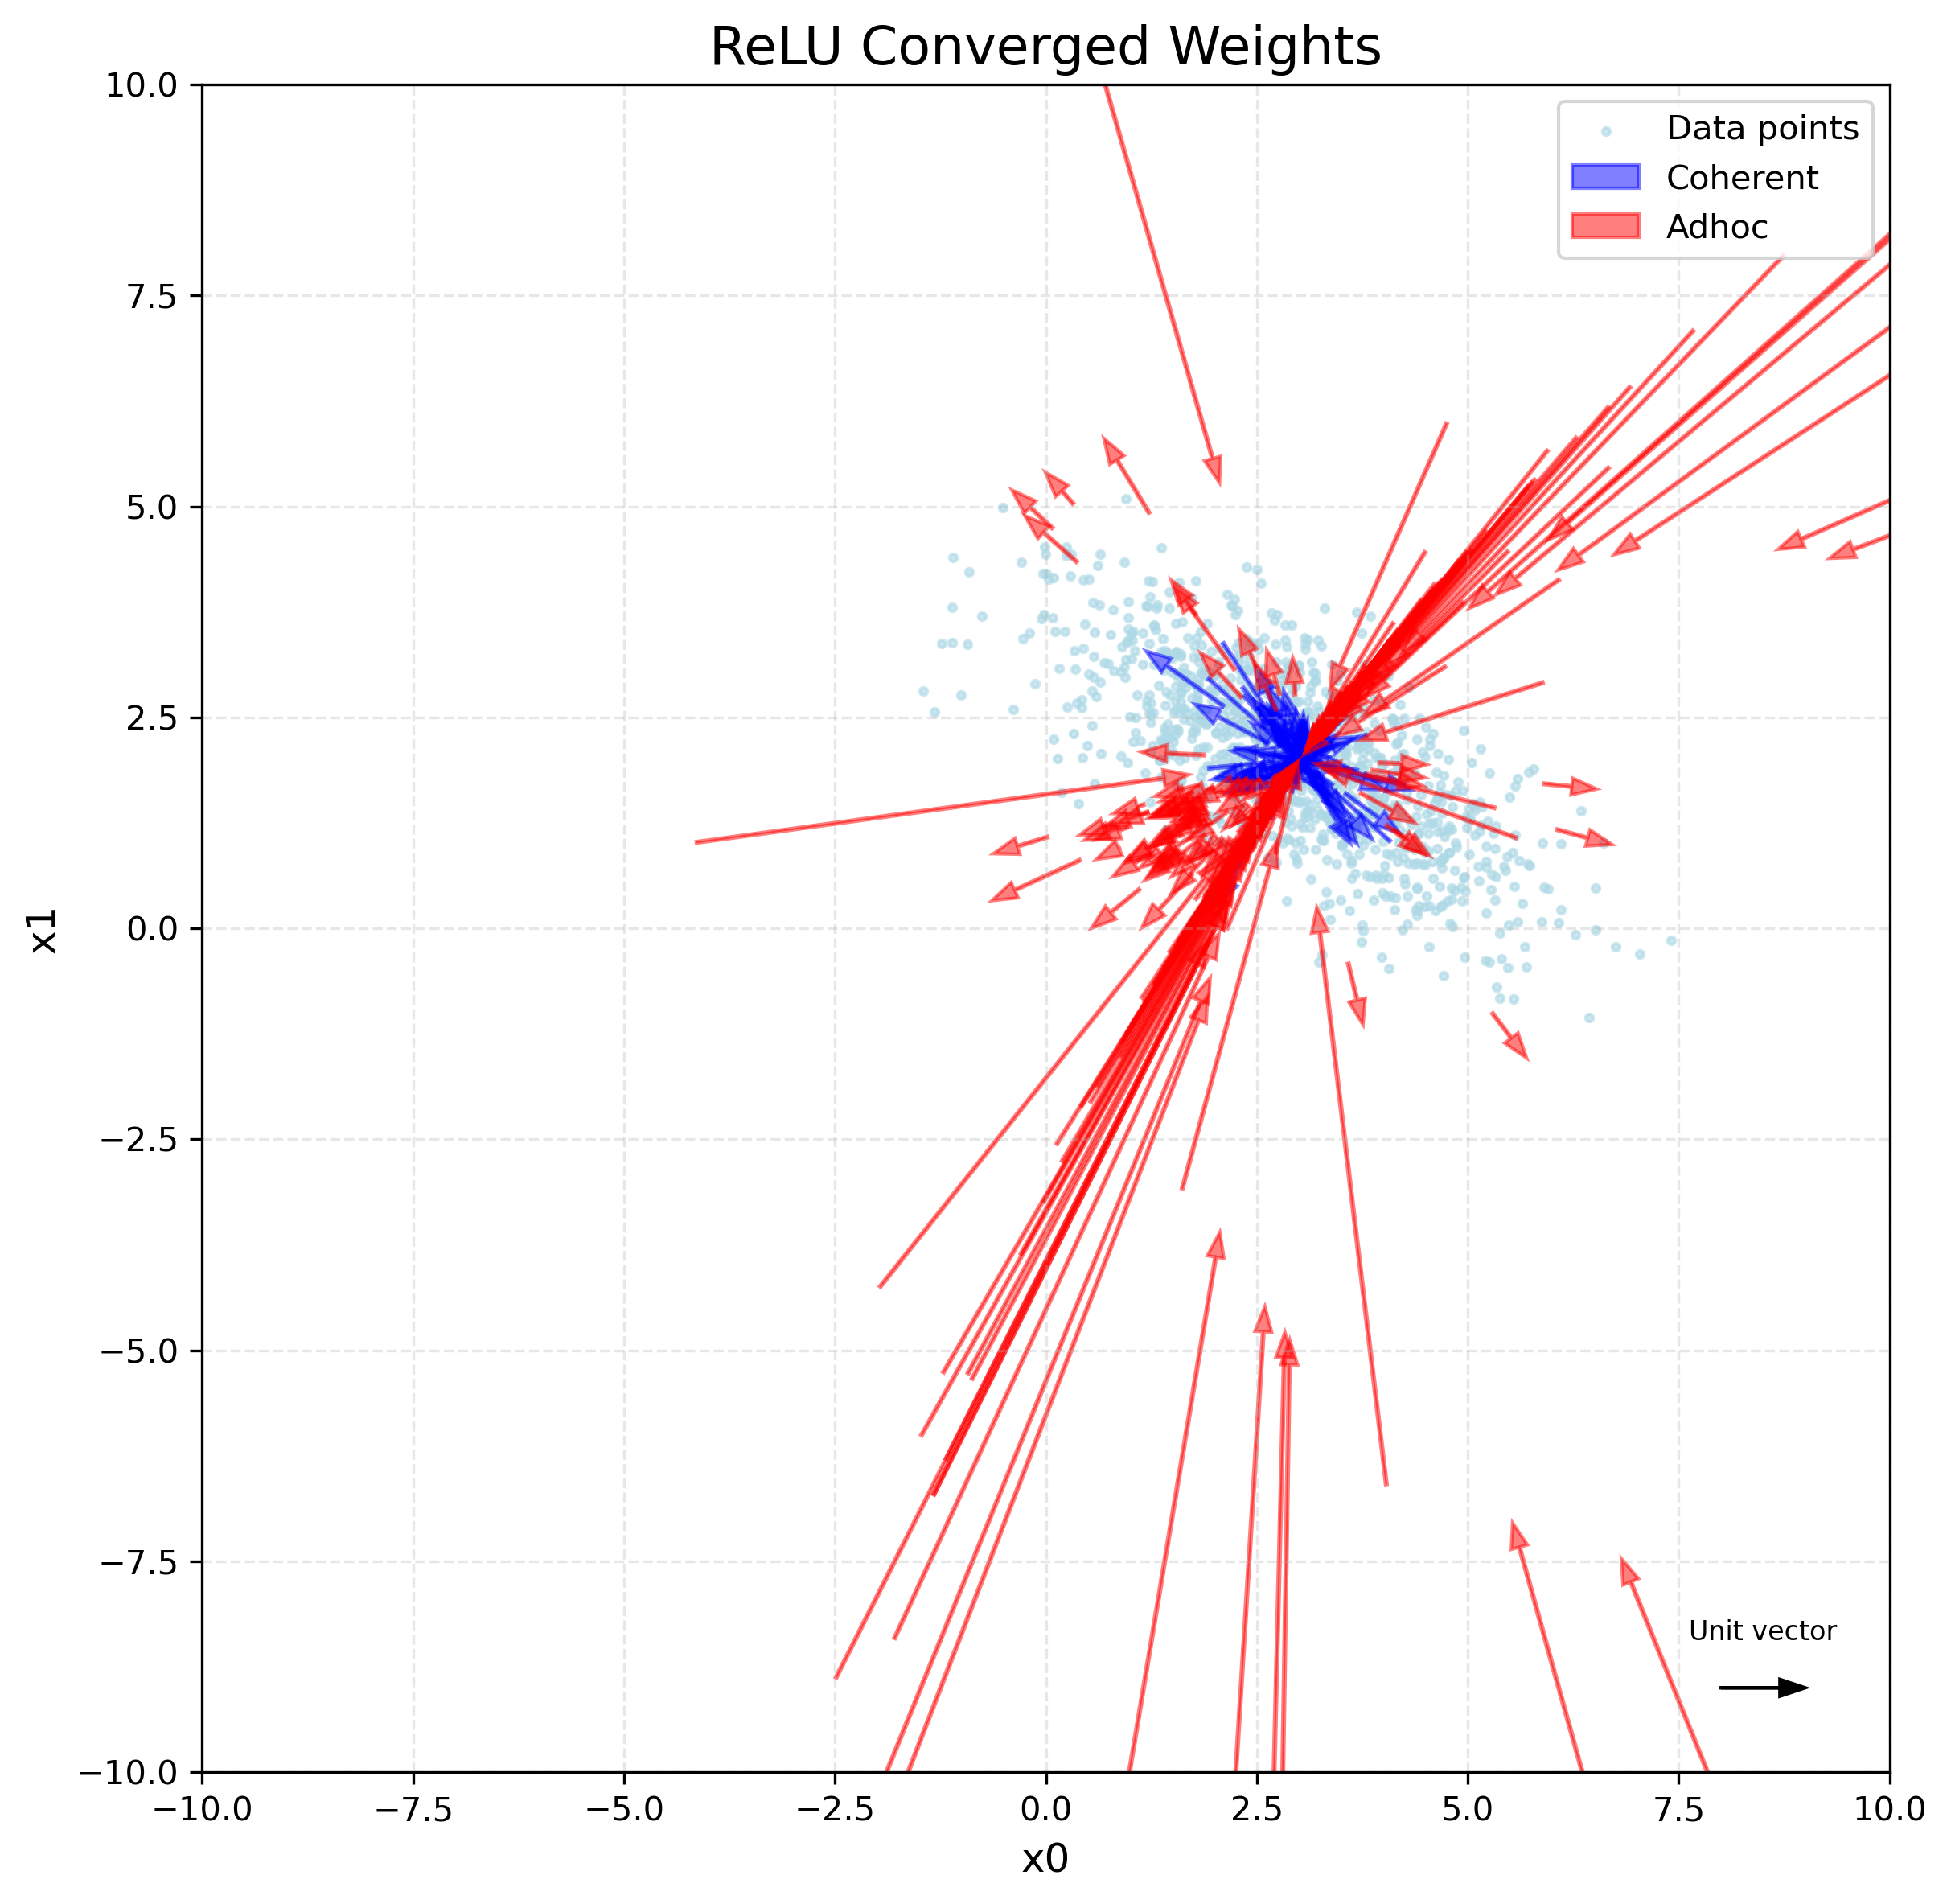
\includegraphics[width=\linewidth]{converged_states_relu.png}
        \caption{ReLU Activation}
        \label{fig:converged_relu}
    \end{subfigure}
    \hfill
    \begin{subfigure}[b]{0.48\textwidth}
        \centering
        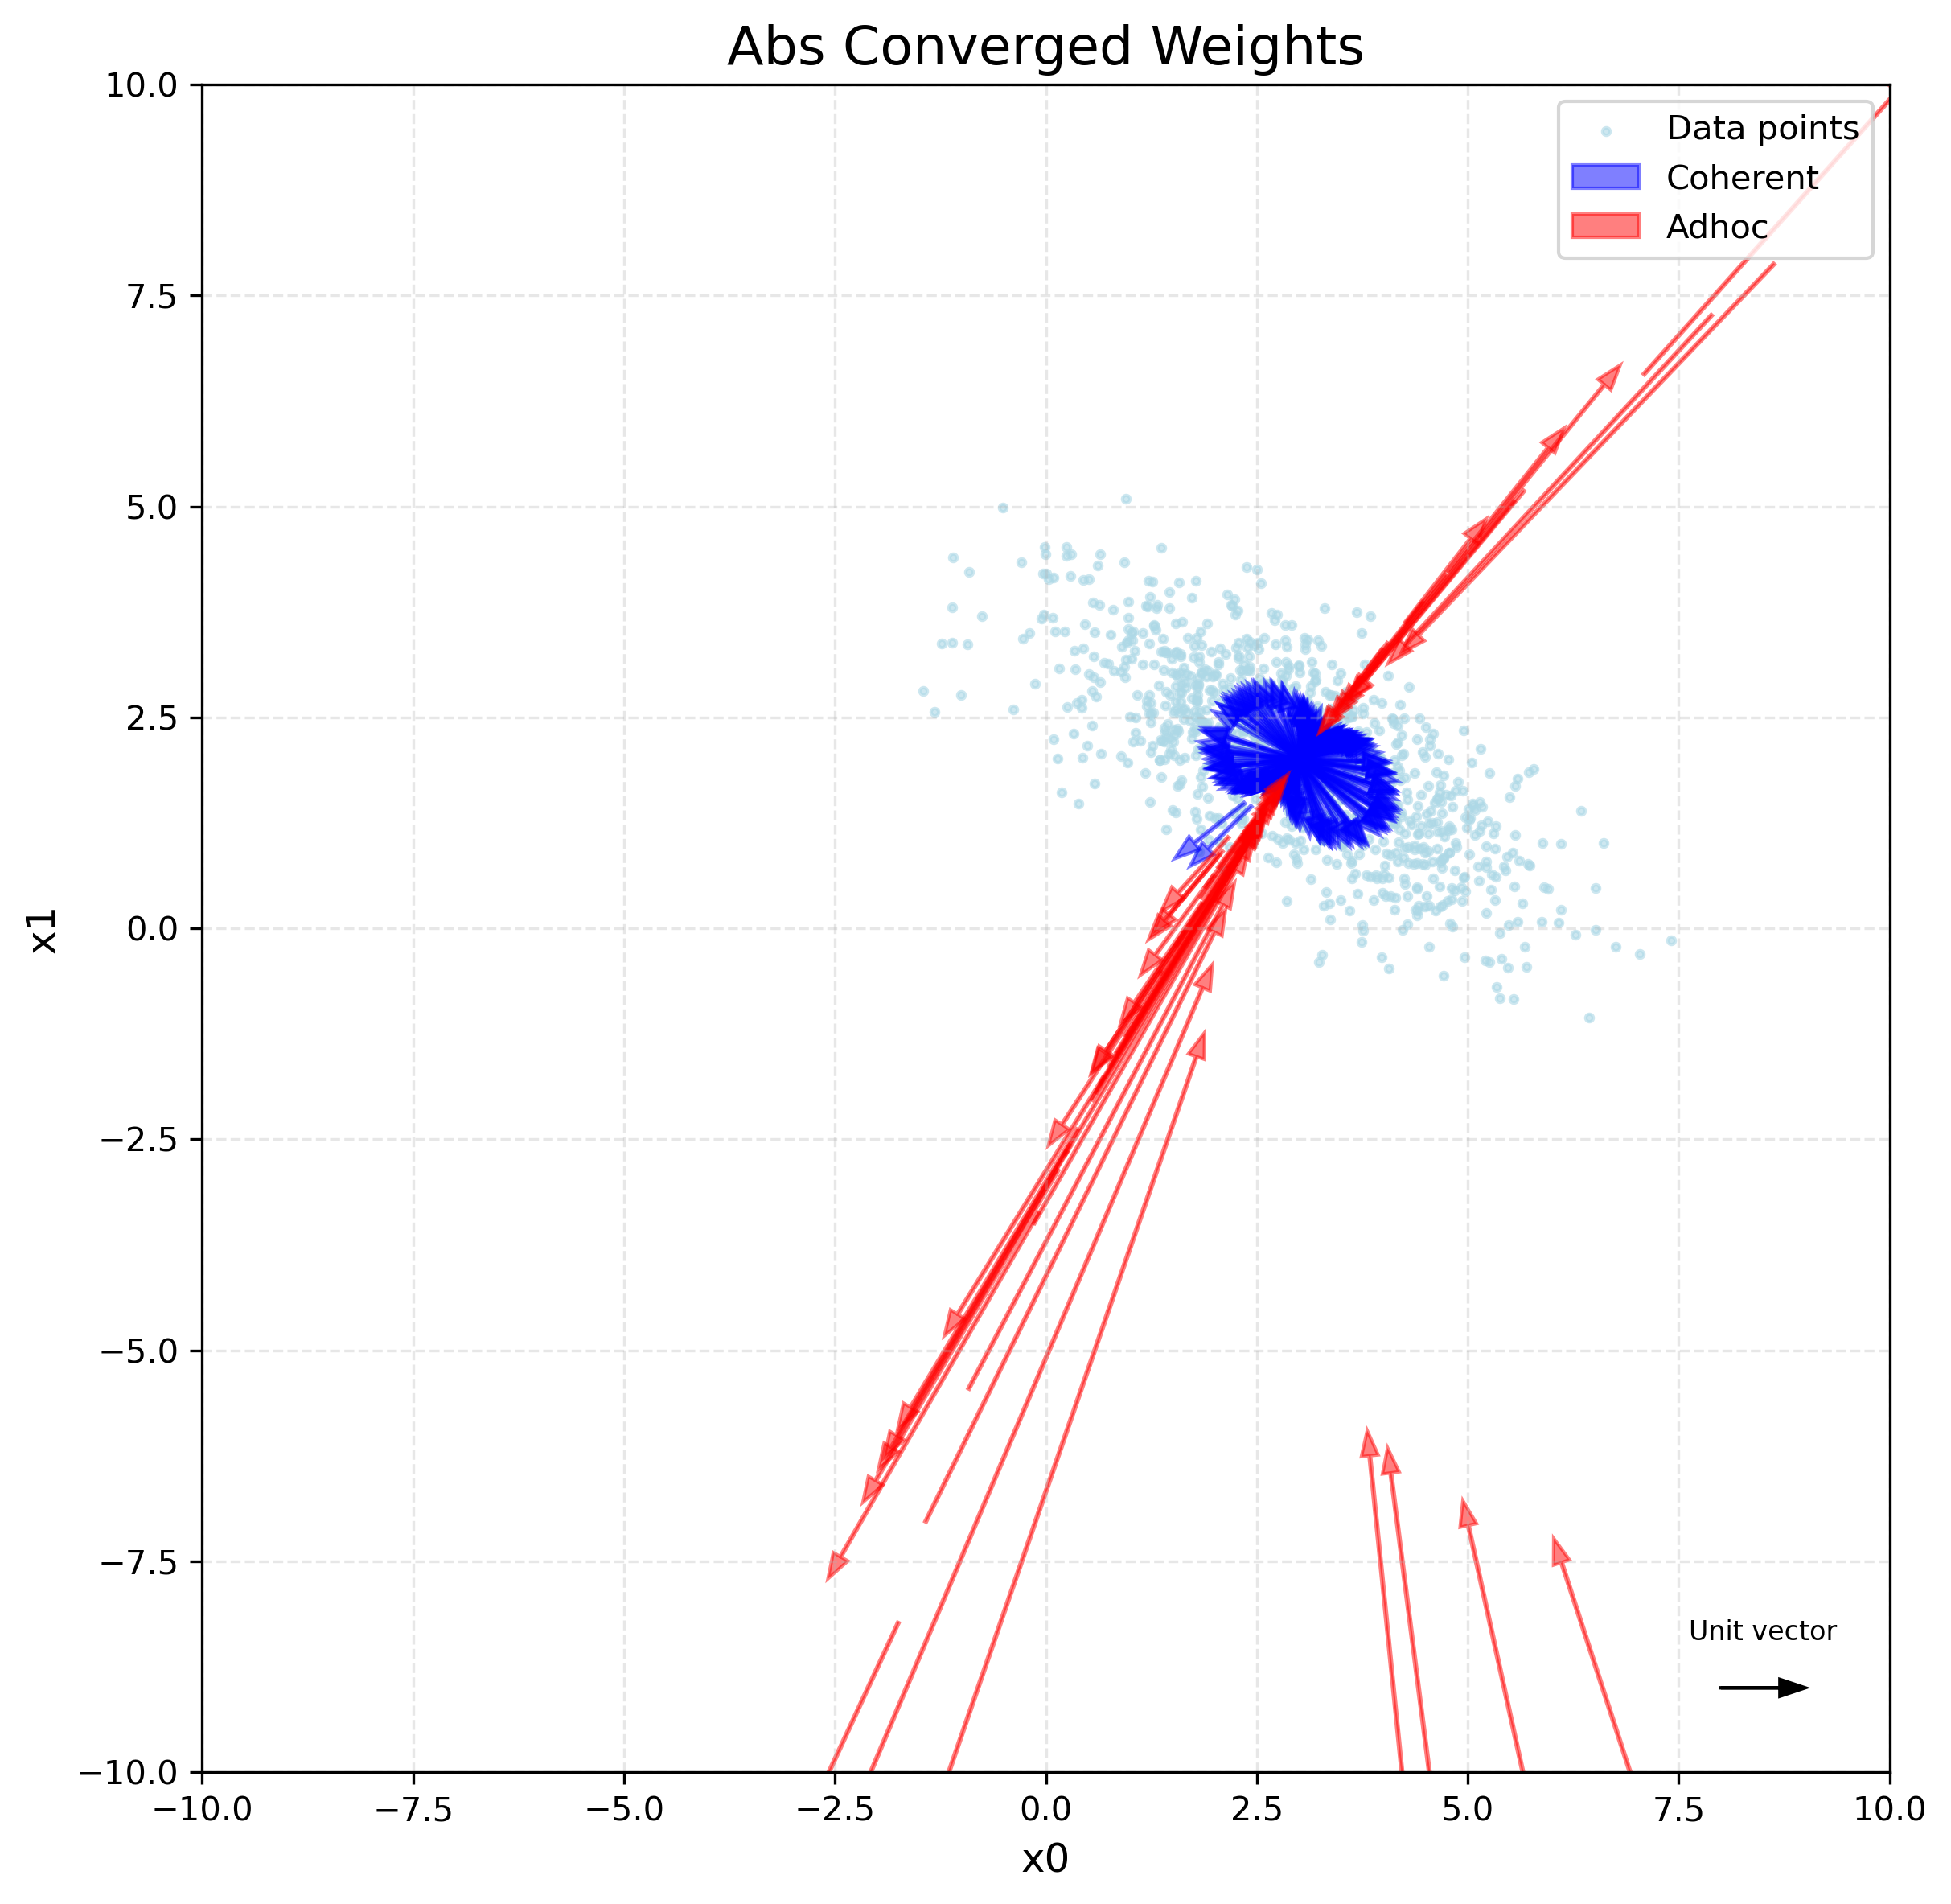
\includegraphics[width=\linewidth]{converged_states_abs.png}
        \caption{Abs Activation}
        \label{fig:converged_abs}
    \end{subfigure}    
    \caption{Converged states for ReLU and Abs activations. The blue dots represent the 2D Gaussian data points. Arrows represent the learned weight vectors originating from the projection of $\boldsymbol{\mu}$ onto the decision boundary. Blue arrows indicate Coherent solutions, and red arrows indicate Adhoc solutions.}
    \label{fig:converged_states}
\end{figure}
    
\subsubsection{Solution Classes: Coherent vs.\ Adhoc}

Upon analysis, we observed that the solutions could be classified into two categories:

\begin{itemize} 
    \item \textbf{Coherent Solutions}: Models where the decision boundary intersects the Gaussian mean $\boldsymbol{\mu}$. These models tend to align with the statistical properties of the data, potentially capturing the principal components. We classified a model as Coherent if the distance between $\boldsymbol{\mu}$ and the decision boundary was less than a small threshold $\epsilon$.
    
    \item \textbf{Adhoc Solutions}: Models where the decision boundary does not intersect $\boldsymbol{\mu}$. These models approximate the target function through other means and may not have an obvious interpretation with respect to the data's statistical properties.
\end{itemize}

\subsubsection{Quantitative Results}

Table~\ref{tab:ex1_stats} summarizes the results of the experiment. The Mean Squared Error (MSE) is reported for both activation functions, along with the counts of models in each solution class.

\begin{table}[h]
    \centering
    \caption{Single Linear Node Results}
    \label{tab:ex1_stats}
    \begin{tabular}{|l|c|c|}
    \hline
    Metric & ReLU & Abs \\
    \hline
    Error & 1.090 & 0.468 \\
    Coherent Error & 0.976 & 0.455 \\
    Adhoc Error & 0.822 & 0.523 \\
    Coherent Count & 4 & 243 \\
    Adhoc Count & 214 & 57 \\
    Dead Count & 82 & 0 \\
    \hline
    \end{tabular}
    \end{table}

\subsubsection{Analysis of Results}

\paragraph{ReLU Activation Models}

As shown in the left image of Figure~\ref{fig:converged_states}, most ReLU models ($214$ out of $300$) resulted in Adhoc solutions. These models tended to align their weights with the dimension of least variance, possibly attempting to minimize error estimating an overall average. The average MSE for ReLU models was higher than that of Abs models, and the Coherent ReLU models had higher error than their Adhoc counterparts.

\paragraph{Abs Activation Models}

The right image in Figure~\ref{fig:converged_states} illustrates the converged states for models with Abs activation. The majority of these models ($243$ out of $300$) produced Coherent solutions, with decision boundaries intersecting near the Gaussian mean. These models exhibited lower average MSE compared to Adhoc Abs models, confirming our hypothesis that Abs activations effectively approximate the Mahalanobis distance by aligning with a mixture of principal components.

However, the Coherent Abs models did not align the largest principal component. While the decision boundary comes very close to the cluster mean, the weights seem to express a mixture of components, as expressed in Equation~\eqref{eq:mixture_pcs}:

\begin{equation} \label{eq:mixture_pcs} \mathbf{W} = \sum_{i=1}^d \alpha_i \mathbf{v}_i^\top, \end{equation}

where $\mathbf{v}_i$ are the principal components and $\alpha_i$ are weighting coefficients. 

The displayed vectors $v / |v|^2|$, seem to form an ellipse or a pair of circles suggesting that $\ell_2(\alpha)=1$ or perhaps that the foci of the Gaussian ellipse have some relationship to the gradient. The exact relationship requires further study. There may be a numerical instability around the direction of least variance that causes the decision boundaries to be ejected from the cluster.

Some of the Adhoc Abs solutions behaved like a ReLU because the Abs function on received inputs on only a single side of the decision boundary. 

\subsubsection{Observations on Initialization and Activation Functions}

The initial weights did not show a clear pattern predicting the solution class into which a model would fall. However, the behavior of the models highlights the importance of the activation function and initialization:

\begin{itemize} 
    \item \textbf{Abs Models Functioning Like ReLU}: The modes where Abs acts like ReLU suggests that proper initialization is crucial for Abs models to capture both sides of the data distribution.
    \item \textbf{ReLU Models Aligning with Least Variance Direction}: The ReLU models often aligned their weights with the smallest principal component, minimizing output the variance across data points. The models are trying to return a constant value, presumably the mean of the target values.
    \item \textbf{Importance of Decision Boundary Placement}: Ensuring that the decision boundary intersects the data cluster increases the likelihood of a model learning a Coherent solution, particularly for Abs activations.
\end{itemize}

\subsection{Conclusion and Next Steps}

The Abs models do not learn principal components directly as we theorized. Instead we discovered a surprising fact about the power of linear units: A single linear unit can estimate the Mahalanobis distance for any dimension Gaussian through principal component mixing.

The findings also reveal the importance of initialization strategies. Abs models that failed to intersect the data cluster tended to behave like ReLU models, resulting in higher error and Adhoc solutions. This suggests that initializing the bias to ensure the decision boundary passes through the data cluster can improve model performance.

\subsection{Data Sampling Initialization}

To address the observations from the initial experiment regarding the importance of the decision boundary intersecting the data cluster, we explored a novel initialization strategy for the bias $b$. Instead of selecting a random point $\mathbf{z}$ from the uniform distribution over $[-8, 8]^2$, we now initialize $b$ using a randomly selected data point $\mathbf{x}_0$ from the dataset $X$. Specifically, we set:

\begin{equation}
b = -\mathbf{W} \mathbf{x}_0,
\end{equation}

ensuring that the initial decision boundary passes through a point within the data cluster. This approach increases the likelihood that the model will capture variations on both sides of the decision boundary, particularly for models using the Abs activation function.

Other than this modification to the bias initialization, all other parameters and settings remain the same as in the initial experiment (see Table~\ref{tab:config_params}).

\subsubsection{Results and Discussion}

Table~\ref{tab:data_init_results} summarizes the results of the experiment using the data sampling initialization strategy.

\begin{table}[h]
    \centering
    \caption{Results with Data Sampling Initialization}
    \label{tab:data_init_results}
    \begin{tabular}{|l|c|c|}
    \hline
    Metric & ReLU & Abs \\
    \hline
    Average MSE (All Models) & 0.833 & 0.407 \\
    Average MSE (Coherent Models) & 1.165 & 0.396 \\
    Average MSE (Adhoc Models) & 0.660 & 0.541 \\
    Number of Coherent Models & 93 & 277 \\
    Number of Adhoc Models & 203 & 23 \\
    Number of Dead Models & 4 & 0 \\
    \hline
    \end{tabular}
\end{table}

Compared to the initial experiment, the data sampling initialization significantly increased the number of Coherent solutions for both activation functions, especially for the Abs models. Specifically, the number of Coherent Abs models increased from 243 to 277 out of 300, while the number of Adhoc Abs models decreased correspondingly.

For the ReLU models, the number of Coherent solutions also increased from 4 to 93, and the number of dead nodes decreased dramatically from 82 to 4. This suggests that initializing the bias using a data point from the dataset effectively activates more ReLU models, allowing them to participate in learning.

\paragraph{Analysis of Abs Models}

The Abs models benefited significantly from the data sampling initialization. The increase in Coherent models indicates that more models had decision boundaries intersecting the data cluster, allowing them to capture variations on both sides of the mean. This led to a slight improvement in the average MSE for Coherent Abs models (from 0.455 to 0.396).

The reduction in the number of Adhoc Abs models further supports the effectiveness of the initialization strategy. With fewer models behaving like ReLU due to all data points being on one side of the decision boundary, the overall performance of the Abs models improved.

\paragraph{Analysis of ReLU Models}

The data sampling initialization led to a significant decrease in the number of dead ReLU nodes, from 82 down to 4. Most of the nodes that were previously dead became Coherent nodes, increasing the number of Coherent ReLU models from 4 to 93 out of 300. This suggests that initializing the bias using data points effectively activates more ReLU models, allowing them to contribute to learning.

While the number of Coherent ReLU models increased, their average MSE also increased (from 0.976 to 1.165). This indicates that although more ReLU models had decision boundaries intersecting the data cluster, they were still limited by the asymmetry of the ReLU activation function, which hinders their ability to approximate the Mahalanobis distance effectively.

The average MSE for Adhoc ReLU models decreased from 0.822 to 0.660. This decrease is noteworthy, but the exact reason is unclear. It may be due to the data sampling initialization producing better Adhoc models; however, further investigation is needed to confirm this. Therefore, we simply note this observation without proposing a specific cause.

\subsubsection{Conclusion of Data Sampling Initialization Experiment}

For the Abs models, this initialization strategy reinforced their ability to approximate the Mahalanobis distance through principal component mixing, as more models aligned their weights with a mixture of principal components.

For ReLU models, while there was an increase in Coherent solutions, their inherent limitations due to the activation function's asymmetry remained evident. 

The data sampling initialization strategy proved effective in increasing the number of Coherent solutions. By ensuring that the decision boundary intersects the data cluster, the models are better positioned to learn representations that capture the statistical properties of the data.

\subsection{Overall Conclusion of Experiment 1}

Experiment 1 reveals that:

\begin{itemize}
    \item Single linear nodes with Abs activation can approximate the Mahalanobis distance of a multivariate Gaussian distribution by learning a mixture of principal components.
    \item We observe two classes of solutions: Coherent units represent deep statistical properies of the data. Adhoc units find solutions that are not deeply grounded in statistical properties.
    \item Initialization strategies that ensure the decision boundary intersects the data cluster enhance the likelihood of models converging to Coherent solutions.
\end{itemize}

Coherent solutions have lower error with Abs. However, this problem was designed for the Abs node to do well on. Coherent solutions in ReLU have higher error, however Abs can be replicated with two ReLU nodes. Additionally, ReLU nodes can also express a signed Mahalanobis distance over [-d..d] using [0..2d] with the next layer accounting for the zero offset. In practice there should not be a huge performance difference between Abs and ReLU.

Adhoc solutions seem to minimize output variance, perhaps attempting to calculate a mean of the target data.

While our initialization strategy increases the change of Coherent features, we don't know that Coherent features are actually beneficial in full models. The next set of experiments, we will investigate whether the benefits of Coherent features and Abs activations persist when applied to the MNIST dataset. This will help determine the practicality and scalability of our approach in more complex scenarios.